


It belongs to the Crouzeix-Raviart family. 
The midside nodes are used as degrees of freedom for the velocities.
It is mentioned in Section~6.3 of \textcite{bobf08} (2008): ``[...]
It is exactly divergence free. Another important feature of this
element is that it can be seen as a "mass conservation" scheme. The present element
has been generalized to second order in \textcite{foso83} (1983).
It must also be said that coerciveness may be a problem for the $P_1^{NC} \times P_0$ 
element, as it does not satisfy the discrete version of Korn's inequality. 
This issue has been deeply investigated and clearly illustrated in \textcite{arno93} (1993).''

\begin{flushright} {\tiny {\color{gray} (tikz\_p1ncp0.tex)}} \end{flushright}
%~~~~~~~~~~~~~~~~~~~~~~~~~~~~~~~~~~~~~~~~~~~~~~~~~~~~~~~~~~~~~~~~~~~~~~~~~~~~~~~~~~~~~~~~~~~~~~~~~~


\begin{center}
\begin{tikzpicture}
%\draw[fill=gray!23,gray!23](0,0) rectangle (5,5);
%\draw[step=0.5cm,gray,very thin] (0,0) grid (5,3.5); %bckgr grid
\draw[thick] (1,0.5) -- (4,1)  -- (3,3) -- cycle; %1-9-2-6-5

%pressure nodes
\draw[violet] (2.75,1.5) circle (4pt); % 0 

%velocity nodes
\draw[black,fill=teal] (2.5,0.75) circle (2pt);
\draw[black,fill=teal] (2,1.75) circle (2pt);
\draw[black,fill=teal] (3.5,2) circle (2pt);

% legend
\draw[black,fill=teal] (3.1,0.2) circle (2pt); \node[] at (3.4,0.2) {$\vec\upnu$};
\draw[violet] (4.1,0.2) circle (4pt); 
\node[] at (4.4,0.2) {$p$};
\end{tikzpicture}\\
\end{center}



At page 170 of \cite{braess} it is stated that ``an analogous quadrilateral element was 
developed and studied by \textcite{ratu92} (1992)''.

In \textcite{bobf13} we find: ``We consider the classical (almost\footnote{What does that mean?!}) 
stable nonconforming triangular 
element introduced in \textcite{crra73}, in which mid-side nodes are used as degrees of 
freedom for the velocities. This generates
a piecewise linear nonconforming approximation; pressures are taken constant on
each element. It is also possible to build a three-dimensional
version of this element, using mid-face nodes as degrees of freedom.''
Also: ``It must also be recalled that coercivity is a problem for the $P_1^{NC}\times P_0$ 
element. The trouble is that the bilinear form (8.2.1) is not coercive on the 
nonconforming space $V_h$ and we do not have the discrete version of Korn's inequality.''

It is also mentioned in \textcite{john16}, appendix B.3, example B.43, in 2D and 3D, 
in \textcite{brfo} (example 8.1), and studied extensively in \textcite{john98} (1998). 

\begin{center}
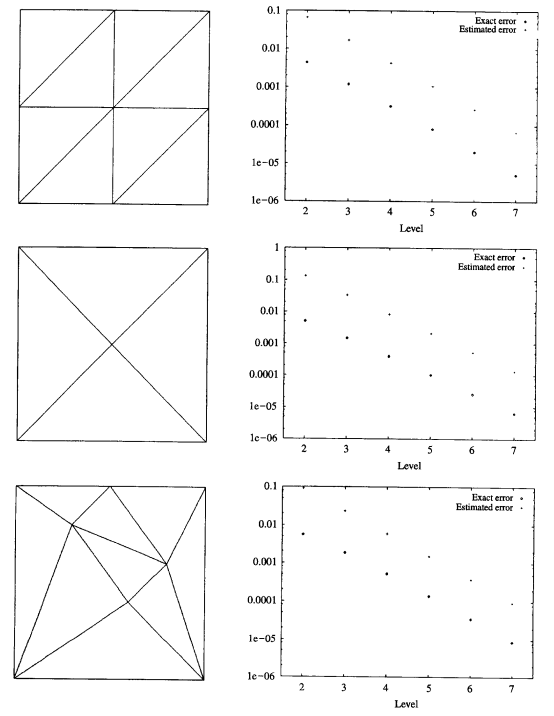
\includegraphics[width=8cm]{images/pair_p1ncp0/john98}\\
{\captionfont Taken from \textcite{john98}.}
\end{center}

In \textcite{jolm17} (2017) the authors show results obtained with this element (fig 6) 
but also explain that these are obtained with so-called reconstructed test functions.
 
